% Copyright (c)  2005-2010 EDF-EADS-PHIMECA.
% Permission is granted to copy, distribute and/or modify this document
% under the terms of the GNU Free Documentation License, Version 1.2
% or any later version published by the Free Software Foundation;
% with no Invariant Sections, no Front-Cover Texts, and no Back-Cover
% Texts.  A copy of the license is included in the section entitled "GNU
% Free Documentation License".
\renewcommand{\filename}{docUC_OVI_RandomMixture.tex}
\renewcommand{\filetitle}{UC : Creation of a Random Mixture}

% \HeaderNNIILevel
% \HeaderIILevel
\HeaderIIILevel


\index{Random Vector!Output random vector}
\index{Distribution!Random Mixture}

The objective of this Use Case is to define the a random vector  as a RandomMixture, which means an affine combination of input random variables :
$$
\displaystyle Y = a_0 + \sum_{i=1}^n a_i X_i
$$
where $(a_i)_{ 0 \leq i \leq n} \in \mathbb{R}^{n+1}$ and $(X_i)_{ 1 \leq i \leq n}$ are some  \emph{independent univariate} random variables.\\

Be careful! This notion is different from the Mixture notion where the combination is made on the probability density functions and not on the univariate random variable :
\begin{itemize}
\item Random Mixture : $Y = a_0 + \sum_{i=1}^n a_i X_i$,
\item Mixture : $p_Y = \sum_{i=1}^n a_i p_{X_i}$, where $p_{X_i}$ is the probability density function of $X_i$ and $\sum_{i=1}^n a_i = 1$.
\end{itemize}

When not precised, the coefficient $a_0$ is taken equal to $0$. Besides, when not specified, the weights $(a_i)_{ 0 \leq i \leq n} $ are taken equal to $1$.\\


Details on each object may be found in the User Manual  (\href{OpenTURNS_UserManual_TUI.pdf}{see User Manual - Probabilistic modeling / Affine combinations of independent univariate random variables}).\\


Open TURNS evaluates the probability density function and cumulative distribution function of the random variable $Y$. So, it is possible to ask $Y$ any request compatible with a {\itshape Distribution} : moments, quantiles, PDF and CDF evaluations, ...\\

It is important to note that the distribution evaluation of $Y$ needs the evaluation of  the characteristic functions of the univariate $X_i$. Open TURNS proposes an implementation of all its univariate distributions, continuous or discrete ones. But only some of the them have the implementation of a specific algorithm that evaluates the characteristic function : it is the case of all the discrete distributions and most of (but not all) the continuous ones. In that case, the evaluation is performant. For the remaining distributions, the generic implementation might be time consuming for high arguments. \\

Furthermore, let's note that as $Y$ is \emph{not} a {\itshape CompositeRandomVector}, it cannot be used by a FORM/SORM algorithm, a QuadraticCumul algorithm or even a Simulation algorithm... In order to use such algorithmes, it is necessary to transform the {\itshape RandomMixture} in a {\itshape CompositeRandomVector} by using the identity function $f : \mathbb{R} \rightarrow \mathbb{R}$ quickly defined (see the following python script).\\

The example here is an output variable of interest defined as the following combination :
$$
Y = 2 + 5X_1 + X_2
$$
where :
\begin{itemize}
\item  $X_1$ follows a $\mathcal{E}xponential(\lambda = 1.5)$,
\item  $X_2$ follows a $\mathcal{N}ormal(\mu = 4,Variance = 1)$.
\end{itemize}

The UC asks $Y$ its mean, variance, probability density graph, quantile of order $90\%$, its probability to exceeds 3.



\noindent%
\requirements{
  \begin{description}
  \item[$\bullet$] none
  \end{description}
}
{
  \begin{description}
  \item[$\bullet$] the random mixture $Y$ : {\itshape myRandomMixtureY}
  \item[type:] RandomMixture
  \end{description}
}

\textspace\\
Python script for this UseCase :

\begin{lstlisting}
  # Create the univariate distributions

  # X1 : Exponential(1.5)
  X1 = Exponential(1.5)
  # X2 : Normal(4,1)
  X2 = Normal(4,1)

  # Put them in a DistributionCollection
  distribList = DistributionCollection( (X1, X2) )

  # Create the numerical of the distribution weights
  # coefficients a1, a2
  weight = NumericalPoint( (5., 1.) )

  # Create the constant coefficient a0
  a0 = 2.0

  # Create the Random Mixture Y = a0 + Sum(ai Xi)
  myRandomMixtureY = RandomMixture(distribList, weight, a0)

  # Or create the Random Mixture where a0 = 0 : Y = Sum(ai Xi)
  myRandomMixtureY = RandomMixture(distribList, weight, a0)

  # Or create the Random Mixture where all the weights (a1, a2)are equal to 1
  myRandomMixtureY = RandomMixture(distribList, a0)

  # Ask myRandomMixtureY its  mean, variance, quantile of order 0.9, its probability to exceeds 3
  mean = myRandomMixtureY.getMean()[0]
  variance = myRandomMixtureY.getCovariance()[0,0]
  quantile90 = myRandomMixtureY.computeQuantile(0.90)[0]
  proba = 1-myRandomMixtureY.computeCDF(3.0)

  # Ask myRandomMixtureY to draw its pdf
  pdfY = myRandomMixtureY.drawPDF()
  # Visualize the graph without saving it
  Show(pdfY)
  # Save it in a file in all formats
  pdfY.draw("pdfY")

  # Transform the RandomMixture into a CompositeRandomVector
  # First, define the identity function : f(x) = x  
  f = NumericalMathFunction('x','x')
  # Then, do the mapping of type
  myRandomVectorY = RandomVector(f,myRandomMixtureY)
\end{lstlisting}





\begin{figure}[H]
  \begin{minipage}{8cm}
    \begin{center}
      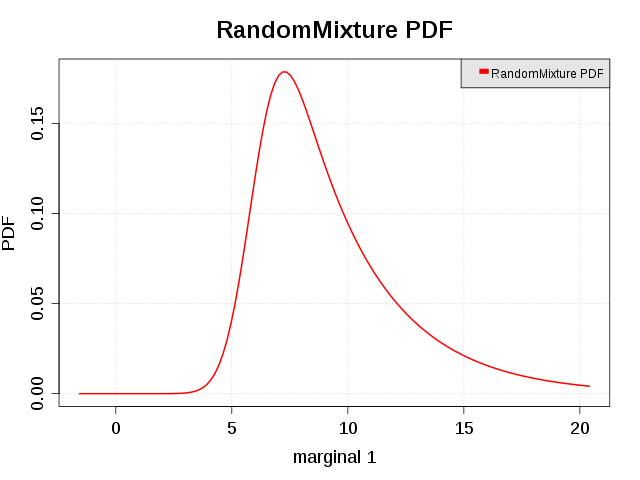
\includegraphics[width=8cm]{RandomMixture_pdf.png}
      \caption{Probability density function of a Random Mixture.}
      \label{PDFRandomMixture}
    \end{center}
  \end{minipage}
  \hfill
  \begin{minipage}{8cm}
    \begin{center}
      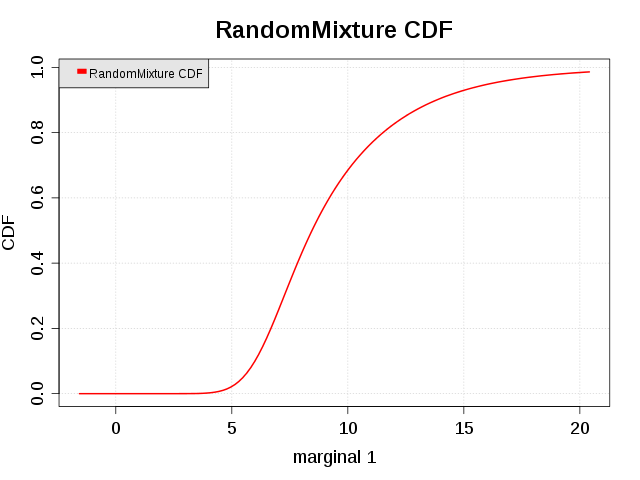
\includegraphics[width=8cm]{RandomMixture_cdf.png}
      \caption{Cumulative density function of a Random Mixture.}
      \label{CDFRandomMixture}
    \end{center}
  \end{minipage}
\end{figure}

